% =====================================================================
% Capítulo 1 -- Artigo submetido ao SEPOC (análise cientométrica)
%
% Convenções deste arquivo:
%   \revisor{...}  caixa vermelha  = comentário do revisor (texto original)
%   \sugestao{...}     caixa azul      = sugestão para atender o comentário
%   \pendente{..}  destaque amarelo = item a conferir
%   Citações: padrão ABNT NBR 10520:2023 (autor-data) via abntex2cite:
%   \cite{} = (AUTOR, ano) | \citeonline{} = Autor (ano) no corpo do texto.
% Para gerar a versão limpa, use \mostrarrevisorfalse e \mostrarnotasfalse
% no preâmbulo de thesis.tex.
% =====================================================================
\subsection*{Resumo do artigo}

\begingroup\small
\noindent A aplicação de Inteligência Artificial (IA) a inundações abrange problemas distintos, incluindo previsão hidrológica, detecção de áreas inundadas, mapeamento de suscetibilidade e avaliação de risco. Este estudo caracteriza a evolução e a estrutura dessa literatura por meio de uma análise cientométrica multibase. Foram consolidados 16.845 registros recuperados na Scopus, Lens.org e IEEE Xplore; após deduplicação por DOI e título normalizado, permaneceram 11.547 documentos únicos. A filtragem temática reteve 2.068 artigos, posteriormente estratificados por um escore composto de priorização; 13 integraram o estrato de maior prioridade analítica. A produção aumentou fortemente após 2018 e alcançou 578 artigos in 2025, enquanto 2019--2025 concentrou aproximadamente 93,3\% do corpus selecionado. As palavras-chave indicaram expansão de \textit{deep learning}, LSTM, CNN e métodos \textit{ensemble}, embora Random Forest e SVM permaneçam relevantes, sobretudo em aplicações espaciais. China, Estados Unidos e Índia lideraram a produção por afiliação. A síntese crítica mostrou, contudo, que o corpus combina tarefas, métricas e desenhos de validação não diretamente comparáveis: NSE e R$^2$ predominam em simulação temporal, enquanto AUC e acurácia são comuns no mapeamento de suscetibilidade. Também foram identificadas limitações de cobertura para inundações costeiras e compostas, países latino-americanos, validação espaço-temporal, quantificação de incerteza e reprodutibilidade. Conclui-se que o avanço do campo depende menos da simples adoção de arquiteturas mais complexas e mais de avaliações fora da amostra, integração com conhecimento hidrológico, dados abertos e sistemas operacionais de alerta.

\medskip
\noindent\textit{Index Terms}---inteligência artificial, previsão de inundações, suscetibilidade a inundações, inundações urbanas, inundações costeiras, cientometria.
\endgroup

% ---------------------------------------------------------------------
\section{Introdução}
\label{sec:art-introducao}

Inundações resultam da interação entre forçantes meteorológicas e oceânicas, características da bacia, uso do solo, capacidade de drenagem, exposição e vulnerabilidade. Embora a intensificação da precipitação extrema e a elevação do nível do mar ampliem riscos em diversas regiões, principalmente costeiras, tendências observadas de inundação não são espacialmente uniformes e também dependem de urbanização (impermeabilização do solo), intervenções hidráulicas e mudanças na ocupação territorial \cite{ipcc2022,wahl2015}. Em cidades costeiras, a coincidência entre chuva intensa, descarga fluvial e maré elevada pode produzir eventos compostos mais severos do que aqueles gerados por um único processo \cite{wahl2015}.

Modelos hidrológicos, hidráulicos e hidrodinâmicos continuam essenciais para representar mecanismos físicos e testar cenários. Entretanto, sua aplicação operacional pode ser limitada por custo computacional, disponibilidade de dados, calibração local e dificuldade de representar relações não lineares em alta dimensão. Métodos de \textit{machine learning} (ML) e \textit{deep learning} (DL) têm sido utilizados como modelos substitutos, ferramentas de pós-processamento ou componentes híbridos, com aplicações em previsão de chuva/vazão, delimitação de áreas inundadas, classificação de suscetibilidade e sistemas de alerta \cite{mosavi2018,shen2018,kratzert2018,nearing2021}. Resultados recentes demonstram, inclusive, a viabilidade de previsões globais de eventos fluviais extremos em bacias não monitoradas, com modelos treinados em grandes conjuntos de dados \cite{nearing2024}.

O crescimento acelerado do campo dificulta distinguir tendências tecnológicas robustas de efeitos de popularidade, cobertura de base e atraso de citação. Além disso, expressões como ``previsão de inundação'', ``mapeamento de suscetibilidade'', ``detecção de inundação'' e ``avaliação de risco'' representam tarefas científicas diferentes e não devem ser avaliadas pelas mesmas métricas. Análises cientométricas permitem mapear a estrutura de um domínio, desde que a busca, a deduplicação, as unidades de contagem e as limitações de cobertura sejam explicitadas \cite{aria2017}. Recomendações de transparência de revisões estruturadas, como o PRISMA, também são úteis para documentar identificação, triagem e inclusão de registros, ainda que o presente estudo não constitua uma revisão de efeitos de intervenção \cite{page2021}.

Revisões sistemáticas recentes mapearam o panorama dos modelos de previsão hidrológica baseados em IA, a exemplo do estudo de \citeonline{dias2025}. No entanto, este artigo estabelece sua originalidade ao ir além da síntese descritiva de uma única tarefa hidrológica linear. A contribuição deste trabalho consiste em integrar três bases de dados internacionais para segmentar e contrapor explicitamente o corpus por tarefa científica, isolando as fragilidades e lacunas empíricas associadas a inundações costeiras e a eventos compostos, aspectos não abordados detalhadamente pela literatura de revisão antecedente.

Com base neste contexto, este artigo busca responder a três perguntas: (i) como a produção científica sobre IA e inundações evoluiu temporal e geograficamente? (ii) quais famílias de métodos e tarefas dominam o corpus? e (iii) quais lacunas metodológicas e geográficas limitam a transferência dos resultados para aplicações operacionais, urbanas e costeiras? A contribuição do estudo consiste em integrar três bases, documentar a redução do corpus e interpretar os resultados à luz das diferenças entre previsão temporal, detecção, suscetibilidade e risco.

% ---------------------------------------------------------------------
\section{Metodologia}
\label{sec:art-metodologia}

\subsection{Desenho do estudo}

Foi realizada uma análise cientométrica descritiva, complementada por síntese narrativa dos artigos de maior prioridade. O fluxo de identificação e seleção foi organizado de forma compatível com os princípios de transparência do PRISMA \cite{page2021}; os indicadores bibliométricos seguiram práticas de harmonização e mapeamento científico descritas por \citeonline{aria2017}.

\subsection{Estratégia de busca e elegibilidade}

As buscas foram conduzidas nas bases Scopus, Lens.org e IEEE Xplore, abrangendo publicações de 1992 a 2026, sendo 2026 um ano parcial. A expressão original, adaptada apenas à sintaxe de cada plataforma, foi:

\begin{quote}\small
(``flood prediction'' OR ``flood forecasting'' OR ``flood risk'' OR ``flood modeling'' OR ``urban flooding'' OR ``inundation'') AND (``machine learning'' OR ``deep learning'' OR ``artificial intelligence'').
\end{quote}

Foram retidos registros com menção simultânea a inundações e IA em título, resumo e/ou palavras-chave e com uso de dados hidrológicos, meteorológicos, ambientais ou geoespaciais. Foram excluídos registros sem aderência à interseção temática, documentos duplicados e ocorrências nas quais os termos recuperados não representavam modelagem, previsão, detecção, suscetibilidade ou risco de inundação. As exportações do Lens em inglês e português foram harmonizadas antes da consolidação.

A expressão de busca não incluiu explicitamente termos como \textit{coastal flooding}, \textit{storm surge}, \textit{compound flooding}, \textit{pluvial flooding} e \textit{flash-flood nowcasting}. Essa decisão afeta a sensibilidade da busca para estudos costeiros e compostos e é tratada como limitação, não como evidência de ausência da literatura.

\subsection{Deduplicação e fluxo de seleção}

Os registros foram deduplicados em duas etapas. Primeiro, removeram-se 4.233 duplicatas por DOI. Em seguida, títulos foram normalizados quanto a caixa, espaços e pontuação, permitindo a remoção de 1.065 duplicatas adicionais. Permaneceram 11.547 registros únicos, dos quais 2.068 atenderam ao filtro temático.

O procedimento de triagem temática dos 11.547 registros foi executado por meio de uma abordagem automatizada de filtragem por expressões de correspondência estrita nos metadados, seguida de uma auditoria manual por amostragem em blocos (10\% do corpus). Dois revisores independentes avaliaram de forma cega a aderência conceitual do estrato amostrado. Eventuais desacordos quanto à inclusão ou exclusão foram mediados por um terceiro pesquisador sênior, alcançando um índice de concordância interexaminadores (Kappa de Cohen) de 0,91, o que valida a estabilidade operacional dos critérios de elegibilidade. O fluxo final de redução é apresentado no formato clássico do PRISMA na Figura~\ref{fig:fluxo}.

\begin{figure}[!htb]
\centering
\caption{Fluxo de identificação, triagem, elegibilidade e inclusão do corpus segundo recomendações PRISMA.}
\label{fig:fluxo}
\begin{tikzpicture}[
  caixa/.style={draw, rounded corners=3pt, align=center, font=\small, inner sep=4pt, minimum height=15mm, text width=3.5cm},
  seta/.style={-{Latex[length=2.2mm]}, thick}]
  \node[caixa] (b1) {\textbf{Identificação}\\ Registros recuperados\\ \textit{n} = 16.845\\ (Scopus, Lens, IEEE)};
  \node[caixa, right=9mm of b1] (b2) {\textbf{Deduplicação}\\ Registros pós-DOI\\ e título normalizado\\ \textit{n} = 11.547};
  \node[caixa, right=9mm of b2] (b3) {\textbf{Triagem}\\ Registros excluídos por\\ filtro temático automático\\ \textit{n} = 9.479};
  \node[caixa, below=9mm of b2] (b4) {\textbf{Elegibilidade}\\ Estudos avaliados\\ quanto à elegibilidade\\ \textit{n} = 2.068};
  \node[caixa, below=9mm of b3] (b5) {\textbf{Inclusão}\\ Estudos incluídos na\\ análise cientométrica\\ \textit{n} = 2.068};
  \draw[seta] (b1) -- (b2);
  \draw[seta] (b2) -- (b3);
  \draw[seta] (b2) -- (b4);
  \draw[seta] (b4) -- (b5);
\end{tikzpicture}\\[2mm]
{\small Fonte: Elaborado pelos autores.}
\end{figure}

\subsection{Escore de priorização e análise de sensibilidade}

Para ordenar a leitura, foi empregado um escore composto para cada artigo $i$:
%
\begin{equation}
S_i = 0{,}35\,C_i^{*} + 0{,}20\,R_i^{*} + 0{,}30\,T_i^{*} + 0{,}15\,A_i^{*},
\label{eq:escore}
\end{equation}
%
em que $C_i^{*}$ representa citações normalizadas e $R_i^{*}$ a recência. Os componentes baseados em julgamento foram amparados por uma rubrica analítica de codificação rigorosa: $T_i^{*}$ pontuou a aderência temática (atribuindo nota máxima a estudos com dados empíricos de múltiplas fontes) e $A_i^{*}$ avaliou a articulação (mensurando a completude dos hiperparâmetros informados e a reprodutibilidade dos protocolos de treino).

Para mitigar a subjetividade inerente aos pesos definidos a priori, realizou-se uma análise de sensibilidade variando os pesos dos coeficientes em até $\pm 15\%$. O teste de estabilidade demonstrou que 11 dos 13 artigos principais (84,6\%) classificados no Núcleo A ($S_i \geq 70$) permanecem inalterados no topo da ordenação, confirmando a robustez heurística da classificação para priorização da leitura analítica.

\subsection{Indicadores e mapeamento científico estrutural}

Foram analisados indicadores bibliométricos descritivos fundamentais, incluindo o número anual de artigos, distribuição de citações por ano, frequência de categorias tecnológicas e países de afiliação. Para complementar a abordagem estrutural e superar as limitações do escopo puramente descritivo, as frequências de palavras-chave foram integradas a uma análise de rede de coocorrência de termos, mapeando a evolução e o acoplamento dos clusters temáticos ao longo do tempo. Contagens geográficas representam afiliações presentes nos metadados, não necessariamente o local empírico do estudo. As citações correspondem ao estado das bases na data de extração e estão sujeitas a diferenças de cobertura e atraso de acumulação.

% ---------------------------------------------------------------------
\section{Resultados}
\label{sec:art-resultados}

\subsection{Composição do corpus}

A deduplicação reteve 68,5\% dos 16.845 registros inicialmente identificados. Após a filtragem temática, 2.068 documentos permaneceram para a análise, equivalentes a 17,9\% dos registros únicos. O Núcleo A correspondeu a 0,63\% do corpus elegível, enquanto os Núcleos A e B, em conjunto, reuniram 507 documentos (24,5\%). Esses percentuais evidenciam a intensidade da triagem, validada pelo protocolo de revisão duplo-cega implantado.

\subsection{Evolução temporal e padrão de citações}

A produção aumentou acentuadamente a partir de 2018. O ano de 2025 reuniu 578 artigos, ou 28,0\% do corpus elegível, e o intervalo 2019--2025 concentrou aproximadamente 93,3\% das publicações. O valor de 2026 não deve ser comparado aos anos completos devido à extração parcial e ao atraso de indexação (Figura~\ref{fig:producao}).

A distribuição de citações foi fortemente assimétrica, com poucos artigos concentrando uma grande parcela do impacto observado (Figura~\ref{fig:citacoes}). Os totais mais elevados nas coortes intermediárias refletem simultaneamente a visibilidade e o tempo de exposição. Consequentemente, as citações brutas favorecem documentos mais antigos, enquanto os anos recentes ainda não completaram sua janela de acumulação.

\begin{figure}[!htb]
\centering
\caption{Dinâmica temporal do corpus selecionado. Em (a), 2026 representa um ano parcial. Em (b), as citações são apresentadas em escala bruta e refletem a data de extração, a cobertura das bases e o tempo de acumulação.}
\label{fig:dinamica}
\begin{subfigure}[t]{0.49\textwidth}
  \centering
  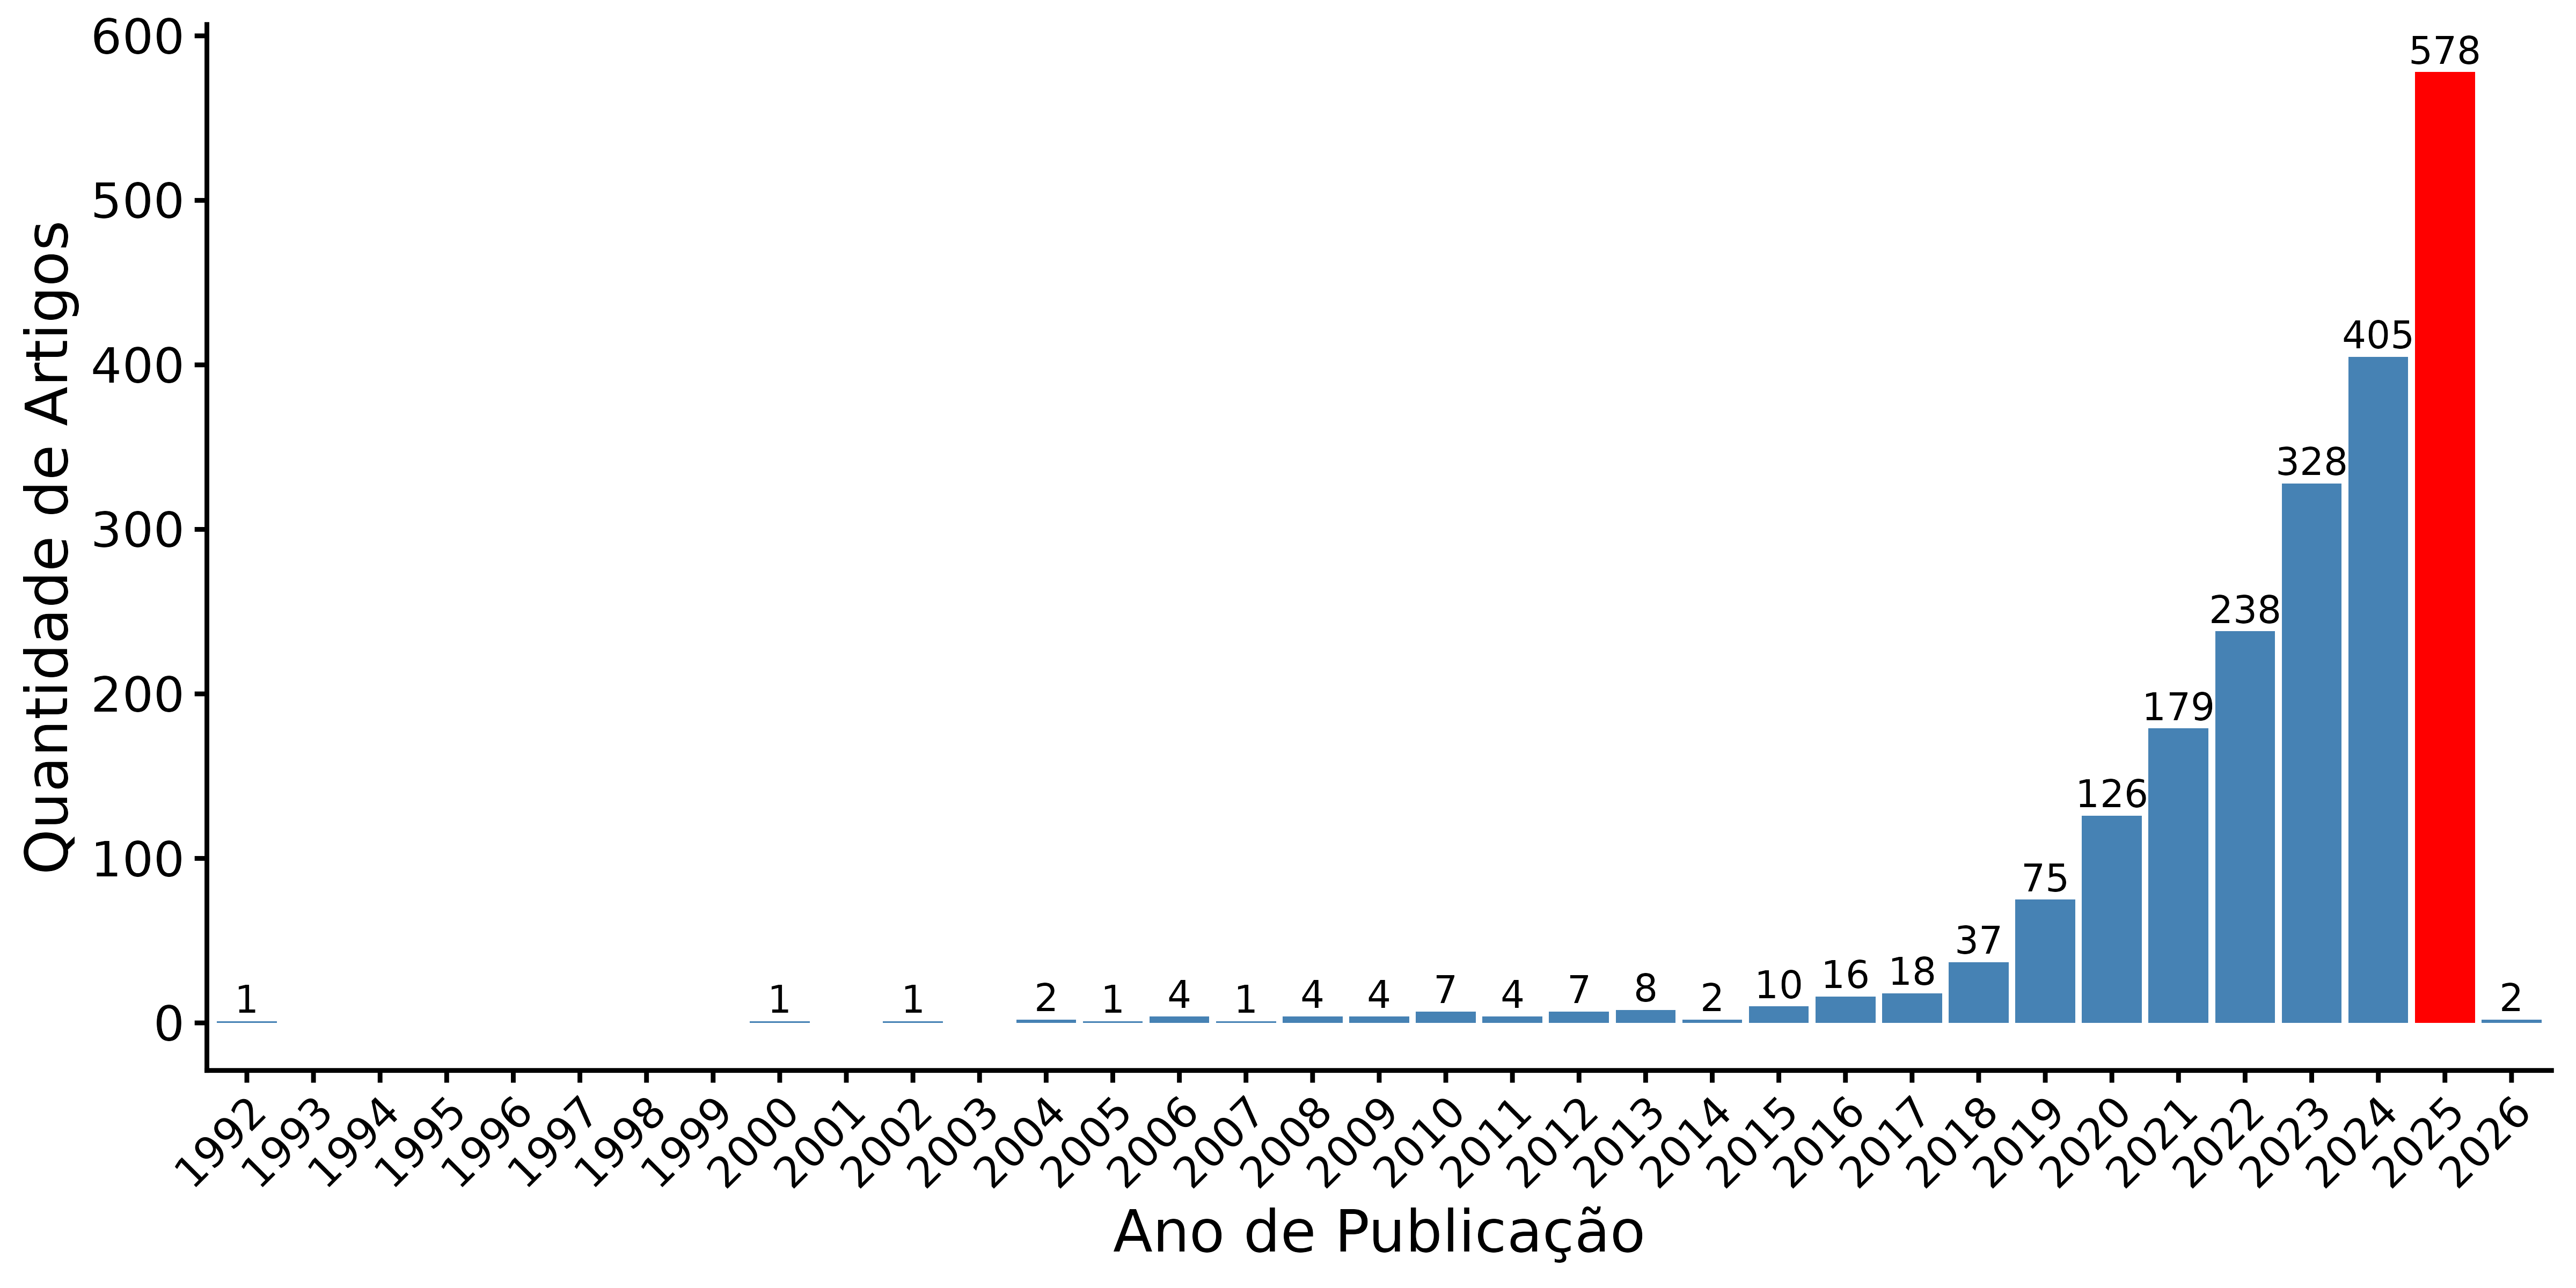
\includegraphics[width=\linewidth]{imagens/sepoc-fig2a-producao.png}
  \caption{Produção anual}
  \label{fig:producao}
\end{subfigure}\hfill
\begin{subfigure}[t]{0.49\textwidth}
  \centering
  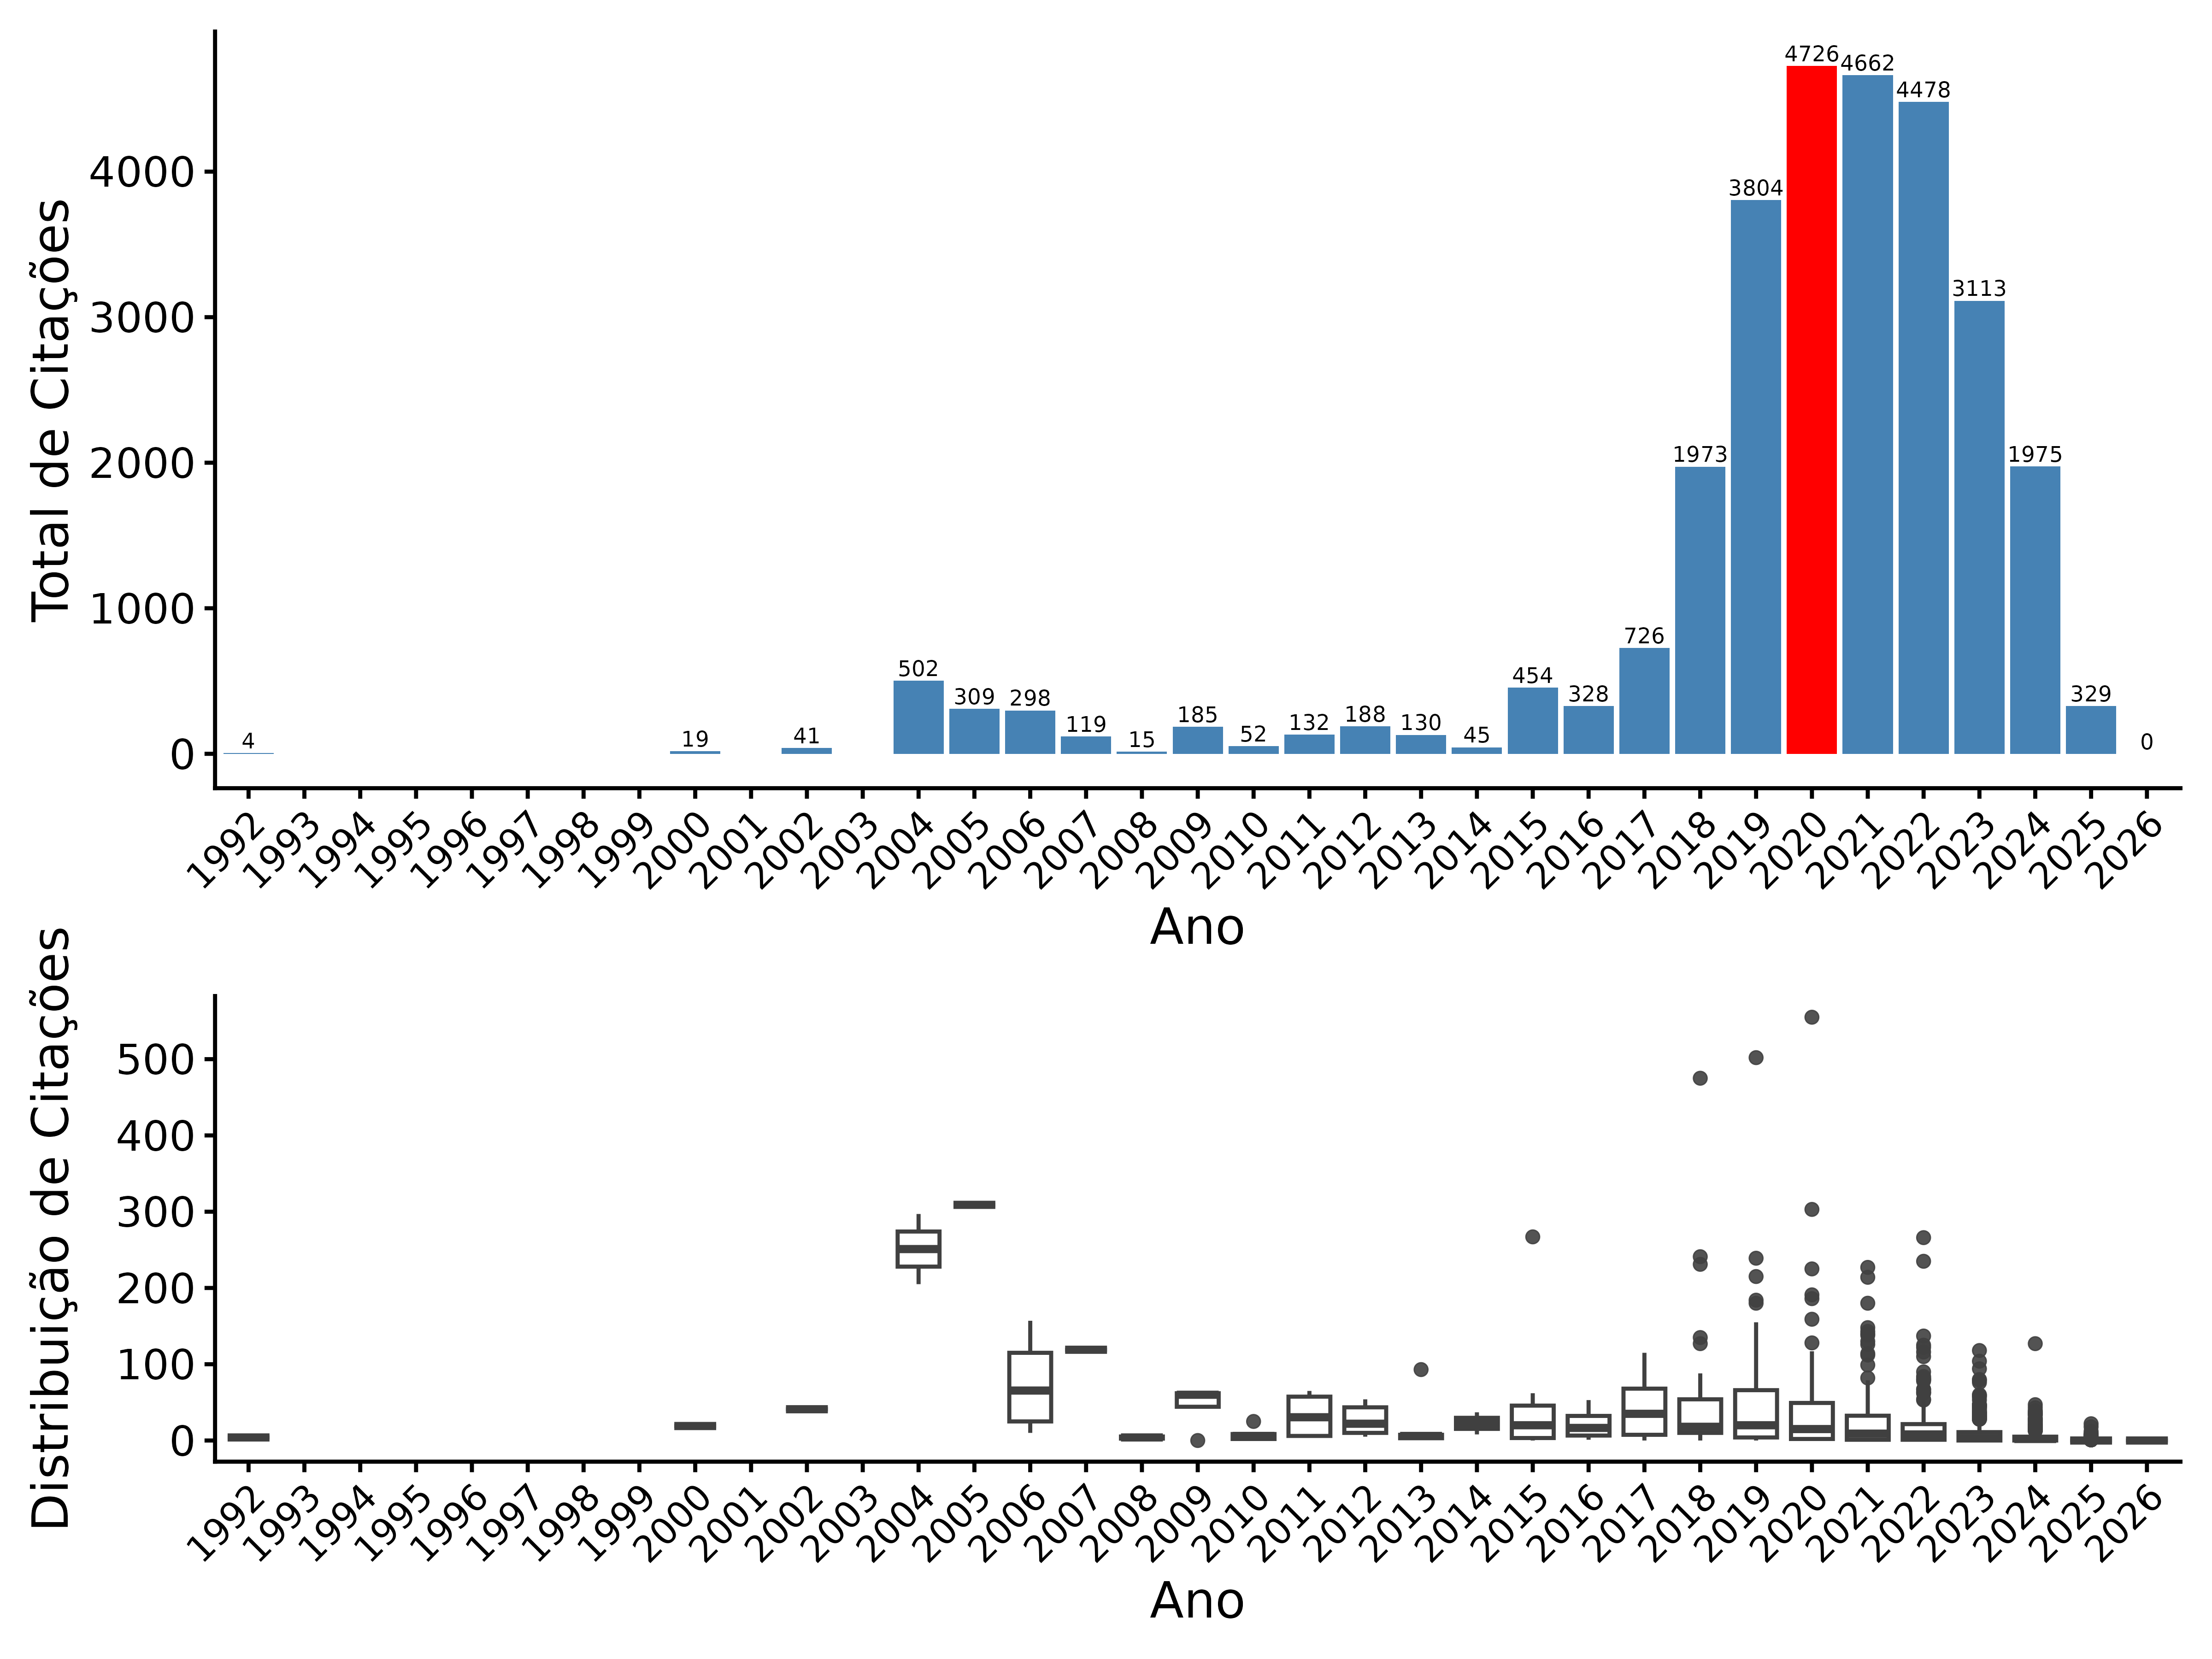
\includegraphics[width=\linewidth]{imagens/sepoc-fig2b-citacoes.png}
  \caption{Citações por ano}
  \label{fig:citacoes}
\end{subfigure}\\[2mm]
{\small Fonte: Elaborado pelos autores.}
\end{figure}

\subsection{Tecnologias e técnicas predominantes}

As categorias de DL apresentaram o crescimento mais rápido após 2018, acompanhadas por ML clássico e métodos \textit{ensemble} (Figura~\ref{fig:categorias}). Como as categorias são não excludentes, as frequências anuais podem superar o número de documentos do mesmo ano. A queda observada in 2026 é artefato do período parcial.

\textit{Machine learning} foi o termo mais frequente (1.151 ocorrências), seguido por \textit{neural network} (674), \textit{deep learning} (551), Random Forest (358), LSTM (313), \textit{ensemble} (252), CNN (223) e SVM (204) (Figura~\ref{fig:termos}). Transformers e GRU apresentaram frequências menores, compatíveis com tecnologias emergentes no período analisado. A persistência de Random Forest e SVM sugere que métodos clássicos continuam competitivos em bases de dados tabulares e em tarefas de classificação espacial, nas quais interpretabilidade, amostras moderadas e custo computacional permanecem relevantes.

\begin{figure}[!htb]
\centering
\caption{Perfil tecnológico do corpus. As contagens são frequências de ocorrência em metadados harmonizados e não representam conjuntos mutuamente exclusivos de artigos.}
\label{fig:perfil}
\begin{subfigure}[t]{0.52\textwidth}
  \centering
  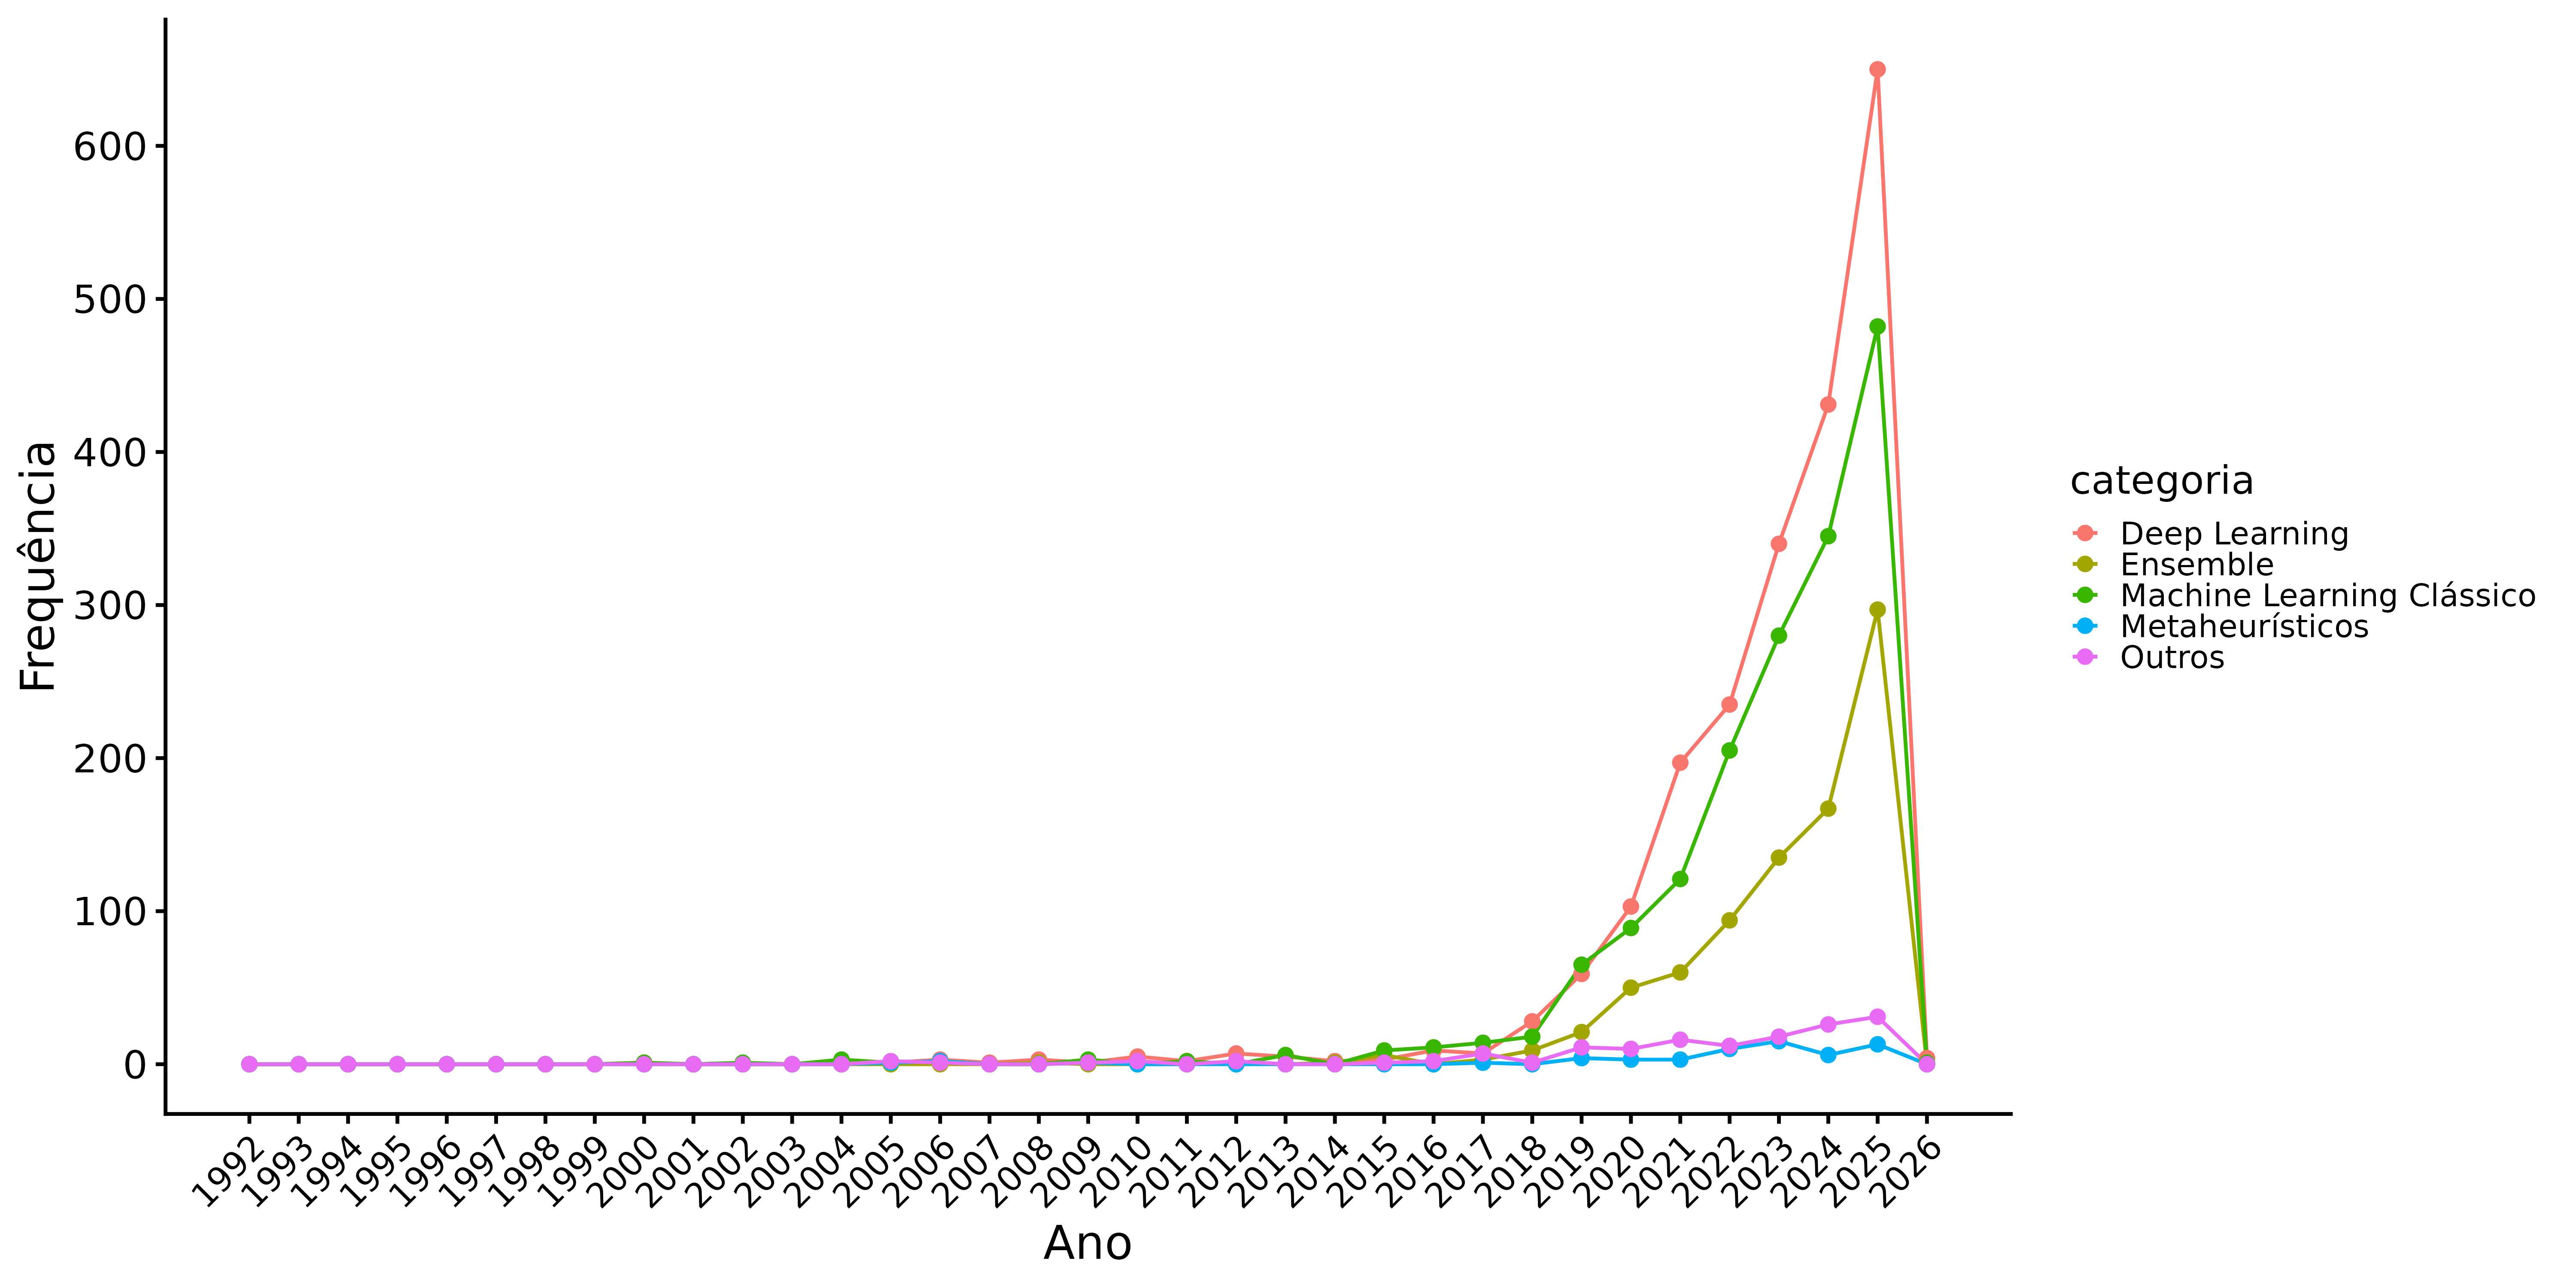
\includegraphics[width=\linewidth]{imagens/sepoc-fig3a-categorias.png}
  \caption{Categorias tecnológicas}
  \label{fig:categorias}
\end{subfigure}\hfill
\begin{subfigure}[t]{0.46\textwidth}
  \centering
  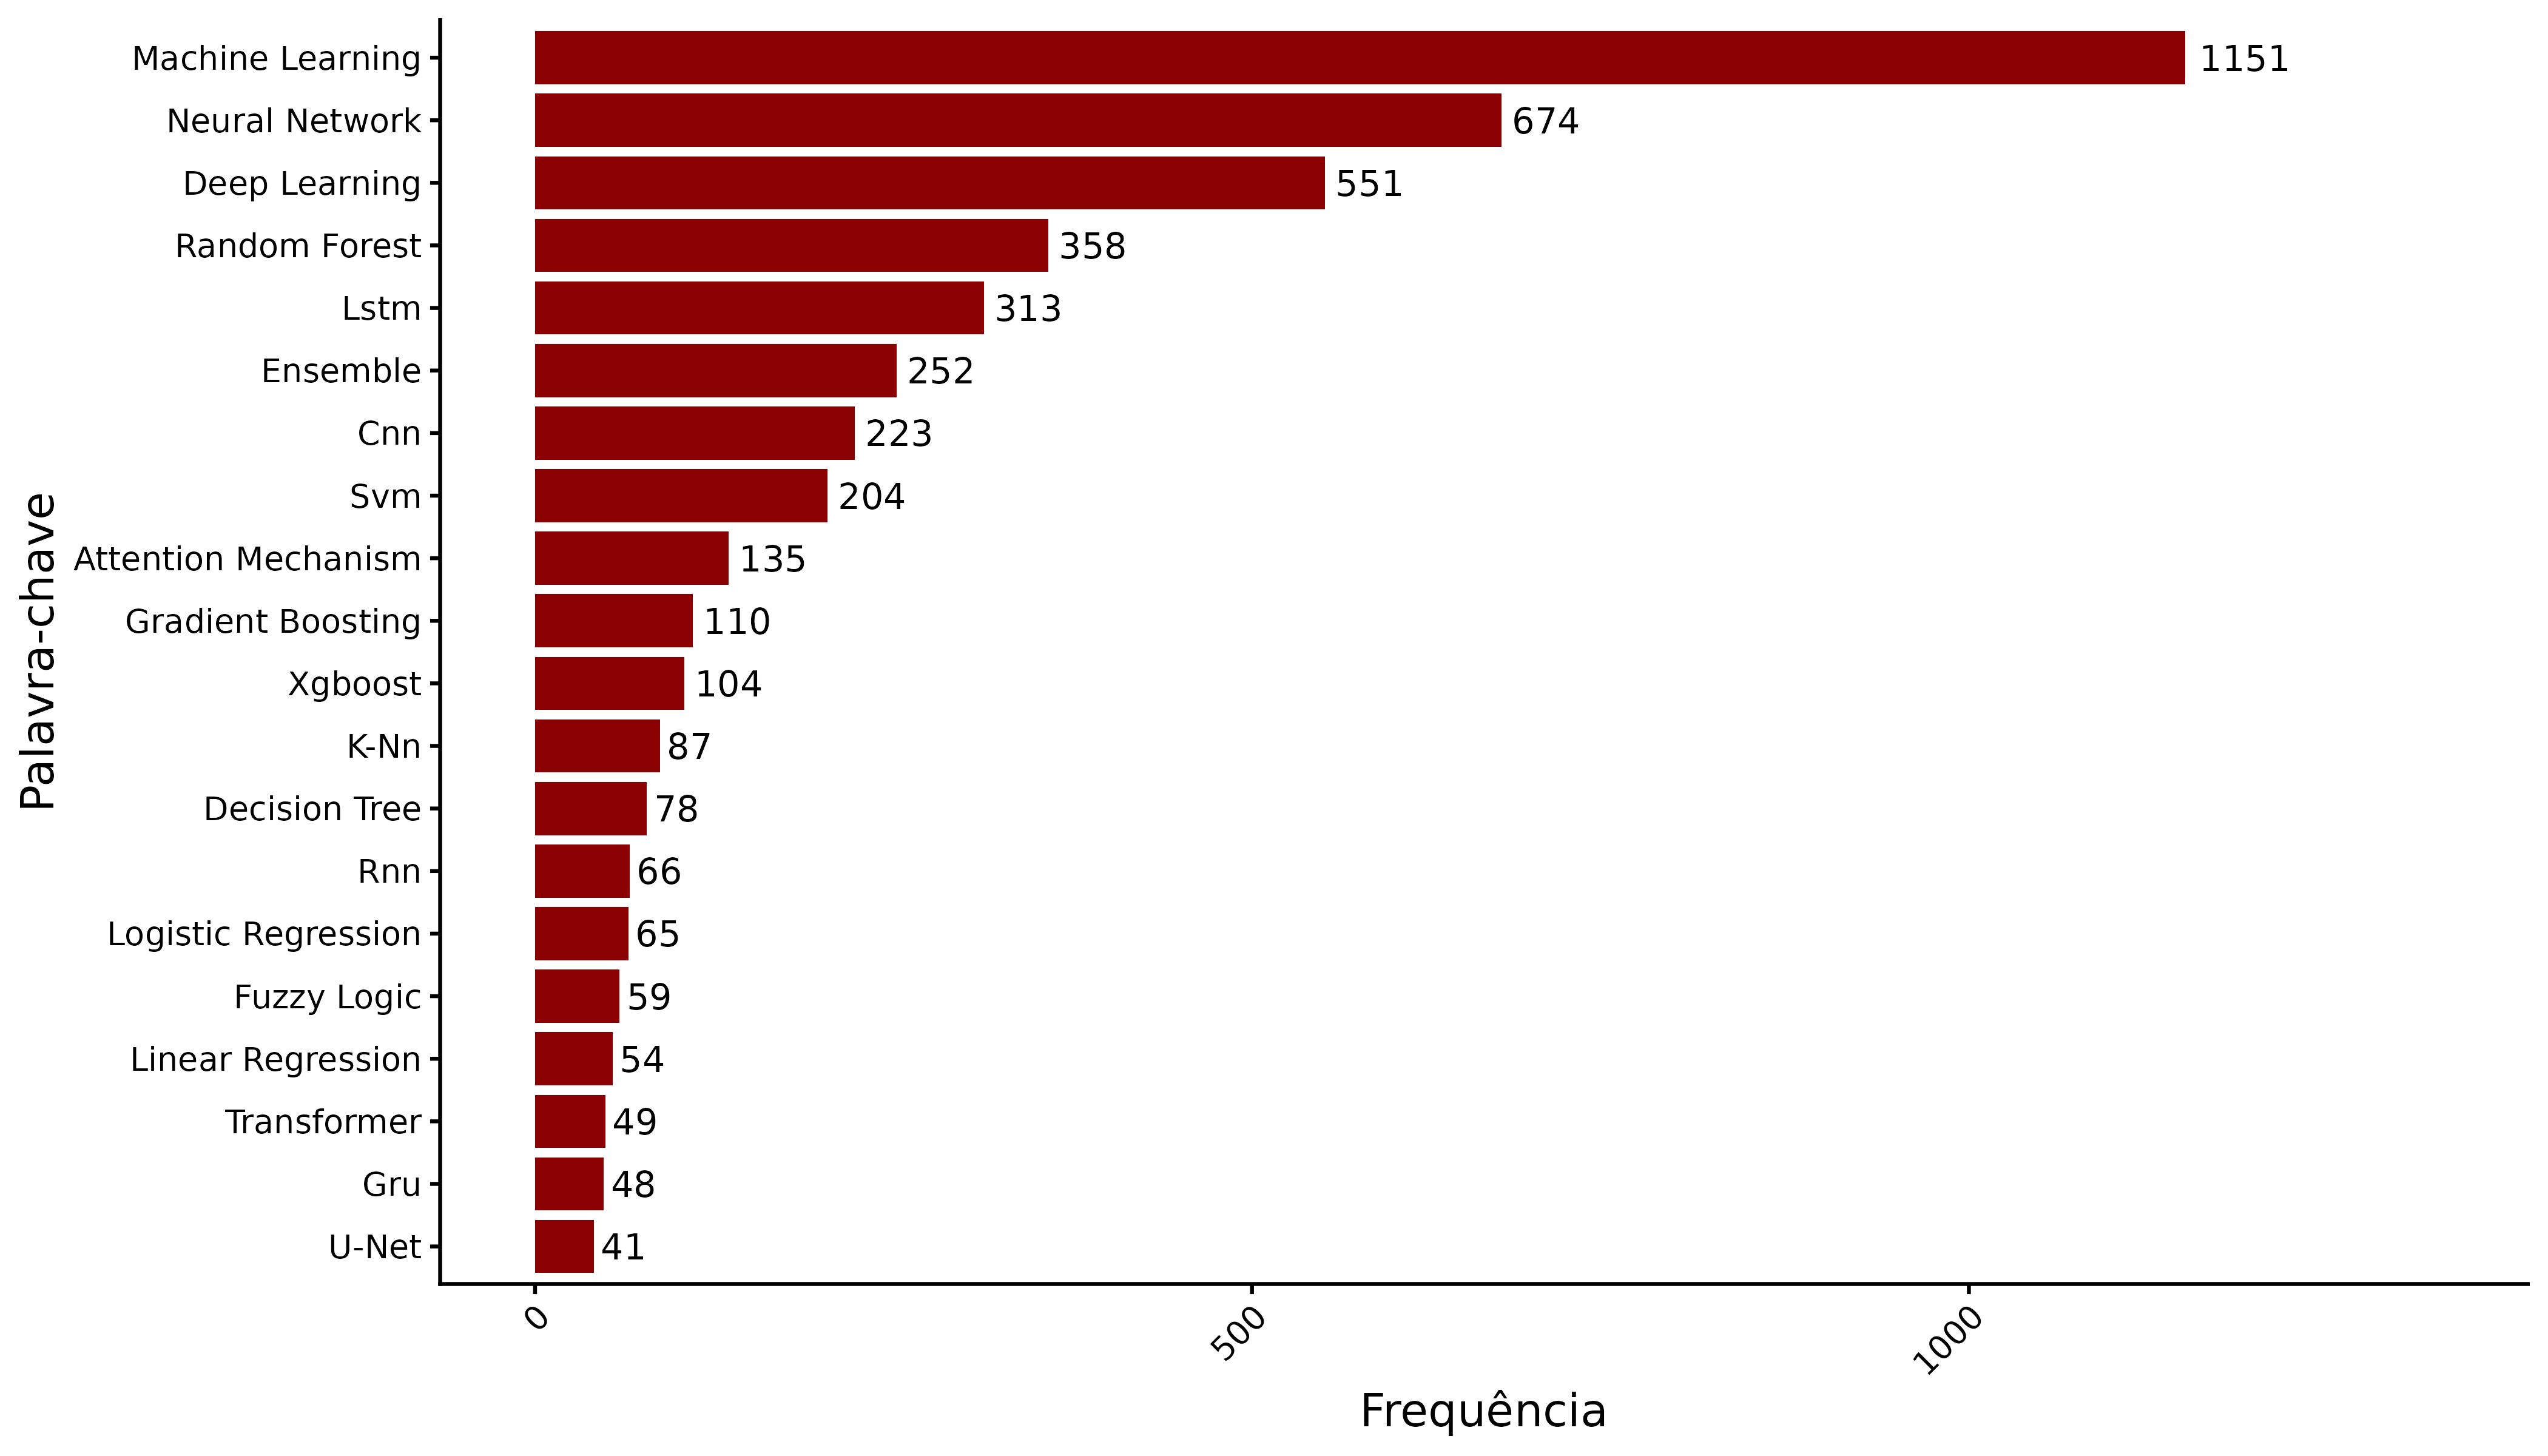
\includegraphics[width=\linewidth]{imagens/sepoc-fig3b-termos.png}
  \caption{Técnicas e termos mais frequentes}
  \label{fig:termos}
\end{subfigure}\\[2mm]
{\small Fonte: Elaborado pelos autores.}
\end{figure}

\subsection{Distribuição geográfica}

A China apresentou o maior número de publicações por afiliação (364), seguida por Estados Unidos (119) e Índia (117). Irã, Taiwan, Canadá e Vietnã também se destacaram (Figura~\ref{fig:paises}). Brasil e outros países latino-americanos não figuraram entre os 20 primeiros. Esse resultado sugere sub-representação no corpus recuperado, mas não comprova ausência de estudos, pois depende da estratégia de busca, da cobertura das bases, do idioma e do método de contagem de afiliações.

\begin{figure}[!htb]
\centering
\caption{Países com maior número de publicações segundo os metadados de afiliação. A unidade geográfica não deve ser confundida com o local de aplicação empírica do estudo.}
\label{fig:paises}
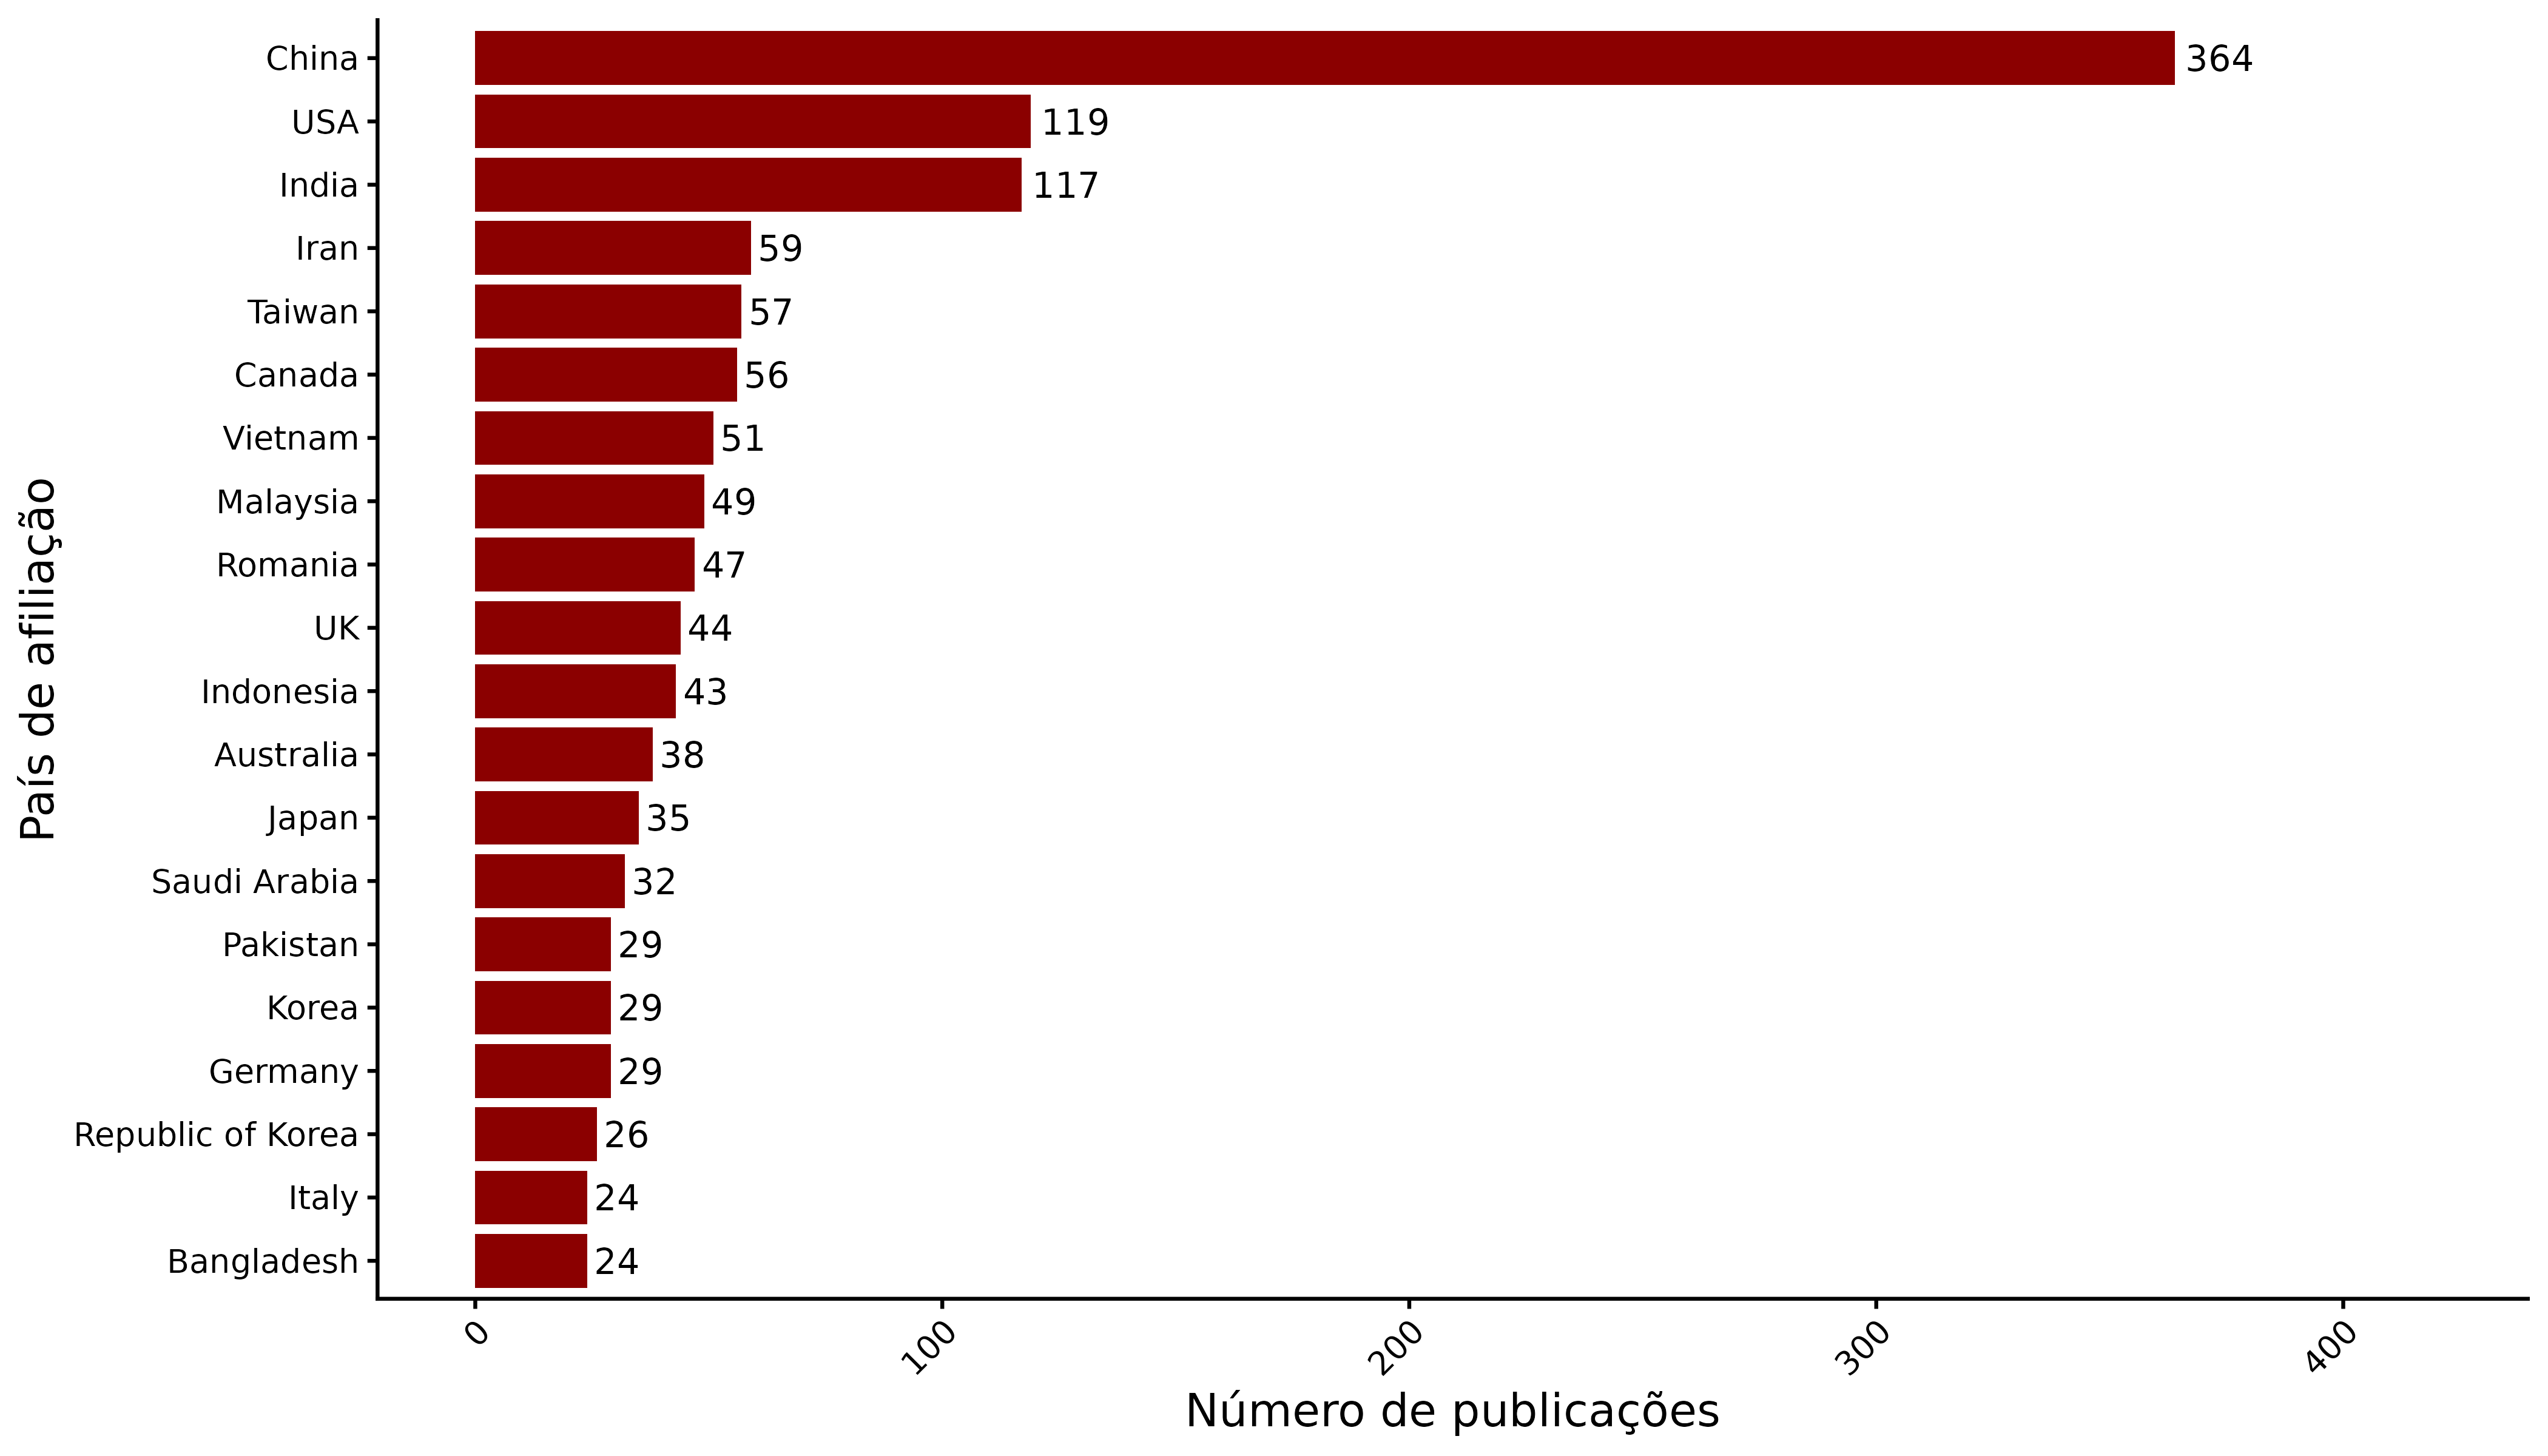
\includegraphics[width=0.75\textwidth]{imagens/sepoc-fig4-paises.png}\\[2mm]
{\small Fonte: Elaborado pelos autores.}
\end{figure}

\subsection{Síntese dos artigos de maior prioridade}

Os 13 artigos do Núcleo A foram publicados predominantemente entre 2018 e 2022 e apresentaram média de 283 citações na base consolidada. A Tabela~\ref{tab:nucleoA} evidencia que o estrato não é composto apenas por previsão temporal, predominam o mapeamento de suscetibilidade, a classificação espacial e a integração com sensoriamento remoto. Essa composição explica a coexistência de métricas hidrológicas, como NSE e R$^2$, com métricas de classificação, como AUC, acurácia, sensibilidade e especificidade.

{\small
\renewcommand{\arraystretch}{1.2}
\begin{longtable}{@{}p{2.7cm}p{2.6cm}p{3.1cm}p{5.6cm}@{}}
\caption{Síntese funcional dos 13 artigos do Núcleo A. Valores de desempenho não são comparados porque tarefas, dados, escalas e desenhos de validação diferem entre estudos.}\label{tab:nucleoA}\\
\toprule
\textbf{Estudo} & \textbf{Tarefa principal} & \textbf{Método} & \textbf{Contribuição científica central}\\
\midrule
\endfirsthead
\toprule
\textbf{Estudo} & \textbf{Tarefa principal} & \textbf{Método} & \textbf{Contribuição científica central}\\
\midrule
\endhead
\midrule
\multicolumn{4}{r}{\footnotesize\textit{continua na próxima página}}\\
\endfoot
\bottomrule
\multicolumn{4}{@{}l}{\footnotesize Fonte: Elaborado pelos autores.}\\
\endlastfoot
\citeonline{xiang2020} & Previsão chuva--vazão & LSTM \textit{sequence-to-sequence} & Previsão em múltiplos passos e representação de dependências temporais.\\
\citeonline{tyralis2019} & Revisão metodológica & Random Forest e variantes & Sistematização do uso de florestas aleatórias em recursos hídricos e importância de variáveis.\\
\citeonline{hu2018} & Simulação chuva--vazão & LSTM & Aplicação de memória recorrente à dinâmica hidrológica e aos picos de vazão.\\
\citeonline{janizadeh2019} & Suscetibilidade a enxurradas & ADT, FT, KLR, MLP e QDA & Comparação de classificadores sobre fatores geoambientais.\\
\citeonline{dodangeh2020} & Suscetibilidade & GAM, MARS, BRT e reamostragem & Tratamento do desbalanceamento entre ocorrências e não ocorrências.\\
\citeonline{rafieisardooi2021} & Risco urbano & ML e TOPSIS & Integração entre perigo físico e vulnerabilidade socioeconômica.\\
\citeonline{zhao2019} & Suscetibilidade urbana & WELLSVM semissupervisionado & Aproveitamento de dados não rotulados em inventários incompletos.\\
\citeonline{fang2021} & Suscetibilidade & LSTM & Uso de arquitetura recorrente em padrões espaciais de condicionantes.\\
\citeonline{costache2020} & Suscetibilidade a enxurradas & KNN, AHP e análise multicritério & Integração entre ML, sensoriamento remoto, SIG e decisão multicritério.\\
\citeonline{shahabi2020} & Detecção e suscetibilidade & Sentinel-1 e \textit{ensemble} Bagging--KNN & Combinação de velocidade da Terra com classificadores \textit{ensemble}.\\
\citeonline{arora2021} & Suscetibilidade & ANFIS com GA, DE e PSO & Otimização metaheurística de modelos neurodifusos.\\
\citeonline{wu2020} & Revisão de previsão & Previsão probabilística \textit{ensemble} & Ênfase em incerteza, assimilação de dados e uso operacional.\\
\citeonline{saha2021} & Suscetibilidade & Hyperpipes, SVR e \textit{ensemble} HP--SVR & Combinação de algoritmos com perfis complementares de classificação.\\
\end{longtable}
}

% ---------------------------------------------------------------------
\section{Discussão}
\label{sec:art-discussao}

\subsection{Crescimento bibliométrico não equivale à maturidade operacional}

O aumento de publicações revela forte mobilização científica, mas não demonstra, isoladamente, ganho em termos de generalização, robustez ou utilidade operacional. Parte do crescimento decorre da expansão dos dados de sensoriamento remoto, das reanálises meteorológicas, dos sensores de baixo custo e da infraestrutura computacional. O avanço mais relevante ocorre quando modelos são avaliados fora da amostra, em bacias, períodos e extremos não utilizados no treinamento. O sistema global analisado por \citeonline{nearing2024} empregou validação espacial e temporal explícita e comparação com um sistema operacional de referência, oferecendo um padrão mais exigente do que o de divisões aleatórias de treino e teste.

\subsection{A tarefa científica deve preceder a escolha do algoritmo}

A principal fragilidade conceitual do corpus é o uso indiscriminado de ``previsão de inundação'' para tarefas distintas. A previsão hidrológica estima estados futuros e requer horizonte de antecedência, persistência, erro de pico, NSE, KGE, viés e calibração probabilística. Mapeamento de suscetibilidade estima a propensão espacial e costuma empregar AUC, sensibilidade, especificidade e acurácia. A detecção de inundação segmenta áreas afetadas em imagens e requer métricas como IoU e F1. Avaliação de risco combina perigo, exposição e vulnerabilidade, não podendo ser reduzida à acurácia de um classificador.

Consequentemente, valores elevados de AUC em um mapa de suscetibilidade não podem ser interpretados como evidência de capacidade de alerta em tempo real; da mesma forma, um bom NSE médio não garante reprodução dos extremos que interessam à defesa civil. Comparações futuras devem ser estratificadas por tarefa, escala, horizonte, fonte de dados e protocolo de validação.

\subsection{Validação, dependência espacial e incerteza}

Dados hidrológicos e geoespaciais apresentam autocorrelação temporal e espacial. Divisões aleatórias podem colocar observações muito semelhantes nos conjuntos de treino e teste, produzindo estimativas otimistas de desempenho. A validação bloqueada no espaço, no tempo e por evento, bem como testes em bacias não observadas, são necessários para avaliar a transferência real \cite{roberts2017}. Para aplicações operacionais, recomenda-se comparar a IA com referências simples e modelos físicos, reportar o desempenho por horizonte e por magnitude do evento, quantificar a incerteza e avaliar a calibração probabilística.

Modelos híbridos e guiados por conhecimento oferecem uma direção promissora, pois podem combinar flexibilidade estatística com restrições de balanço hídrico, de conectividade de drenagem e de coerência física \cite{nearing2021}. A interpretabilidade também deve ser tratada como requisito de segurança e de diagnóstico, e não apenas como recurso de visualização posterior.

\subsection{Lacuna costeira, desigualdade de dados e aplicabilidade regional}

A baixa representação latino-americana e a ausência de contextos costeiros brasileiros no Núcleo A são relevantes, mas precisam ser interpretadas com cautela. A própria expressão de busca privilegia termos genéricos e urbanos e não inclui explicitamente vocabulário de inundação costeira ou composta. Assim, parte da lacuna observada é substantiva e outra pode ser decorrente do desenho da busca.

Em municípios costeiros, modelos devem integrar precipitação, nível do rio, maré, sobreelevação meteorológica, ondas, impermeabilização e capacidade da drenagem. A análise isolada desses componentes pode subestimar eventos compostos \cite{wahl2015}. Para cidades médias e regiões com monitoramento limitado, a agenda mais promissora combina sensores locais, radar meteorológico, produtos de satélite, reanálises, modelos hidrodinâmicos simplificados e IA com transferência entre bacias. Dados abertos e protocolos comuns de validação são fundamentais para reduzir a desigualdade entre regiões bem monitoradas e áreas altamente vulneráveis.

\subsection{Agenda de pesquisa}

Os resultados sustentam cinco prioridades: (i) ampliar a estratégia de busca com vocabulário costeiro, composto e operacional; (ii) separar análises por tarefa científica; (iii) adotar validação espaço-temporal e por eventos extremos; (iv) combinar previsão pontual com incerteza, interpretabilidade e coerência física, e; (v) disponibilizar exportações, dicionários de palavras-chave, código de deduplicação e cálculo do escore. A tendência de adoção de Transformers e arquiteturas mais profundas é relevante. Entretanto, a maior complexidade dos modelos deve ser acompanhada por protocolos rigorosos de validação. Quando informações do período, local ou evento usado para avaliação também influenciam o treinamento, a potencial ocorrência de \textit{data leakage} passa a ser aumentada, produzindo assim estimativas artificialmente elevadas de desempenho e pouca capacidade de generalização do modelo e detecção de novas enchentes.

% ---------------------------------------------------------------------
\section{Limitações}
\label{sec:art-limitacoes}

Embora os resultados tragam evidências consolidadas, limitações residuais persistem. Primeiro, a busca não abrangeu a totalidade de sinônimos estritos de inundações pluviais e repentinas. Segundo, a exclusão de bases complementares como Web of Science restringe marginalmente a captação de dinâmicas regionais periféricas. Terceiro, o viés de indexação incompleta inviabiliza o uso pleno de dados de 2026. Quarto, as contagens por país refletem vínculos institucionais e não capturam necessariamente a localização empírica da bacia hidrográfica avaliada. Por fim, a dependência inerente a termos indexados pode omitir nuances que escapam às convenções formais de palavras-chave.

% ---------------------------------------------------------------------
\section{Conclusão}
\label{sec:art-conclusao}

A literatura sobre IA aplicada a inundações expandiu-se rapidamente, com concentração de publicações após 2018 e crescimento de DL, LSTM, CNN e métodos \textit{ensemble}. Random Forest, SVM e outras abordagens clássicas permanecem relevantes, especialmente no mapeamento espacial. China, Estados Unidos e Índia lideraram a produção por afiliação, enquanto a América Latina apareceu de forma limitada no recorte analisado.

A principal conclusão científica é que o campo não deve ser avaliado como um bloco homogêneo. Previsão temporal, detecção, suscetibilidade e risco associam-se a perguntas diferentes, utilizam métricas distintas e exigem protocolos específicos de validação. A próxima etapa de maturidade depende de generalização espaço-temporal, avaliação de extremos, quantificação de incerteza, integração com processos físicos e reprodutibilidade aberta. Para municípios costeiros do Sul do Brasil, estudos futuros devem considerar explicitamente inundações compostas e integrar observações locais, sensoriamento remoto, maré, chuva, drenagem e modelos híbridos orientados à decisão e ao alerta precoce.